\newpage
\subsubsection{Swellpro Spry+}
\begin{wrapfigure}{r}{0.3\textwidth}
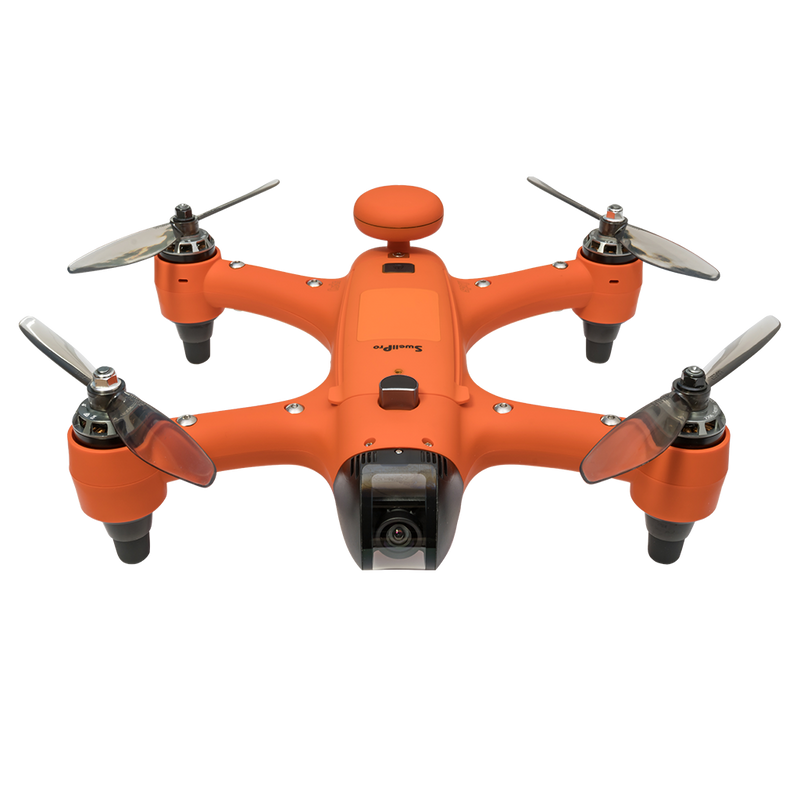
\includegraphics[width=1\linewidth]{uav/models/21_spry.png}
\caption{Spry+}
\end{wrapfigure}
The Spry+ \cite{spry} is Swellpro's action drone. It is also fully designed to be used in the water.

\paragraph{Payload capacity}\mbox{Score: 0} \\
While the payload capacity of the Spry+ is not presented on the website, professionals state that the drone can carry up to 300g\cite{sprypayload}. This is below the minimum required payload of 500g.

\paragraph{Mounting clearance}\mbox{Score: 0.8} \\
The Spry+ is a compact drone meant for speed and therefore lacks clearance for sensors. One could create their own platform beneath the drone, utilizing the four bars.

\paragraph{Navigation/Routing}\mbox{Score: 1.4} \\
One can plan routes for the Spry+ using the SwellPro Spry App. The app has support for waypoint mission planning.

\paragraph{Flight time}\mbox{Score: 1.5} \\
The flight time of the SplashDrone 4 is 15 minutes, passing the minimum required flight time.

\paragraph{Range}\mbox{Score: 0} \\
The maximum radio range is 800m, failing the minimum required range.

\paragraph{Waterproof}\mbox{Score: 1.5} \\
The drone is IP67 waterproof, meaning the drone is dust-tight and can immerse up to 1 meter in water. This is well over the minimum required IP rating.

\paragraph{Landing in water}\mbox{Score: 1.5} \\
The drone is designed to land and take off in the water.

\paragraph{Maneuverability}\mbox{Score: 1.5} \\
The drone can fly horizontally 18m/s. It is designed for high speed movement.

\paragraph{Total score:}\mbox{0} \\
Due to the Spry+ being an action drone it wasn't able to meet the range and payload capacity requirements.

